% ============================================================================
% PROMPT WARS: THE ARENA — Platform Overview for Management
% GLITCH TECH FEST 2026
% ============================================================================
\documentclass[11pt, a4paper]{article}

\usepackage[utf8]{inputenc}
\usepackage[T1]{fontenc}
\usepackage[margin=2cm]{geometry}
\usepackage{xcolor}
\usepackage{titlesec}
\usepackage{enumitem}
\usepackage{booktabs}
\usepackage{array}
\usepackage{tabularx}
\usepackage{fancyhdr}
\usepackage{hyperref}
\usepackage{tikz}
\usetikzlibrary{shapes.geometric, arrows.meta, positioning, calc,
                decorations.pathreplacing, backgrounds, fit}
\usepackage{tcolorbox}
\tcbuselibrary{skins}
\usepackage{float}
\usepackage{parskip}
\usepackage{needspace}
\usepackage{etoolbox}

% --- Tighten spacing ---
\raggedbottom
\setlength{\parskip}{0.3em}
\renewcommand{\topfraction}{0.95}
\renewcommand{\bottomfraction}{0.95}
\renewcommand{\textfraction}{0.05}
\renewcommand{\floatpagefraction}{0.85}
\setcounter{topnumber}{4}
\setcounter{bottomnumber}{4}
\setcounter{totalnumber}{8}

% --- Colours ---
\definecolor{primaryblue}{HTML}{1A3C6E}
\definecolor{accentgold}{HTML}{D4A843}
\definecolor{sectionblue}{HTML}{2C5F9E}
\definecolor{lightgray}{HTML}{F2F2F2}
\definecolor{darktext}{HTML}{2C2C2C}
\definecolor{alertred}{HTML}{C0392B}
\definecolor{successgreen}{HTML}{27AE60}
\definecolor{warnamber}{HTML}{F39C12}
\definecolor{infopurple}{HTML}{8E44AD}
\definecolor{softcyan}{HTML}{2980B9}
\definecolor{rosepink}{HTML}{E74C3C}
\definecolor{monggreen}{HTML}{47A248}

\hypersetup{
    colorlinks=true, linkcolor=sectionblue, urlcolor=sectionblue,
    pdftitle={Prompt Wars Platform --- Management Brief},
}

% --- Header / Footer ---
\pagestyle{fancy}
\fancyhf{}
\fancyhead[L]{\small\textcolor{primaryblue}{\textbf{GLITCH TECH FEST 2026}}}
\fancyhead[R]{\small\textcolor{primaryblue}{Prompt Wars --- Platform Overview for Management}}
\fancyfoot[C]{\small\textcolor{gray}{\thepage}}
\fancyfoot[R]{\small\textcolor{gray}{Confidential --- Internal Review}}
\renewcommand{\headrulewidth}{0.8pt}
\renewcommand{\footrulewidth}{0.4pt}
\renewcommand{\headrule}{\hbox to\headwidth{\color{primaryblue}\leaders\hrule height \headrulewidth\hfill}}
\renewcommand{\footrule}{\hbox to\headwidth{\color{gray}\leaders\hrule height \footrulewidth\hfill}}

% --- Section Styles ---
\titleformat{\section}
  {\large\bfseries\color{primaryblue}}
  {\thesection.}{0.5em}{}[\vspace{-0.4em}\textcolor{accentgold}{\rule{\textwidth}{1.2pt}}]
\titlespacing*{\section}{0pt}{1em}{0.4em}

\titleformat{\subsection}
  {\normalsize\bfseries\color{sectionblue}}
  {\thesubsection}{0.5em}{}
\titlespacing*{\subsection}{0pt}{0.6em}{0.2em}

\pretocmd{\section}{\needspace{4\baselineskip}}{}{}
\pretocmd{\subsection}{\needspace{3\baselineskip}}{}{}

% --- Boxes ---
\tcbset{
    keybox/.style={
        colback=lightgray, colframe=primaryblue, boxrule=0.7pt, arc=3pt,
        left=8pt, right=8pt, top=5pt, bottom=5pt,
        fonttitle=\small\bfseries\color{white}, coltitle=white,
        colbacktitle=primaryblue, toptitle=2pt, bottomtitle=2pt,
        before skip=0.4em, after skip=0.4em,
    },
    greenbox/.style={
        colback=successgreen!6, colframe=successgreen, boxrule=0.7pt, arc=3pt,
        left=8pt, right=8pt, top=5pt, bottom=5pt,
        fonttitle=\small\bfseries\color{white}, coltitle=white,
        colbacktitle=successgreen, toptitle=2pt, bottomtitle=2pt,
        before skip=0.4em, after skip=0.4em,
    },
    purplebox/.style={
        colback=infopurple!6, colframe=infopurple, boxrule=0.7pt, arc=3pt,
        left=8pt, right=8pt, top=5pt, bottom=5pt,
        fonttitle=\small\bfseries\color{white}, coltitle=white,
        colbacktitle=infopurple, toptitle=2pt, bottomtitle=2pt,
        before skip=0.4em, after skip=0.4em,
    },
    amberbox/.style={
        colback=warnamber!6, colframe=warnamber!80!black, boxrule=0.7pt, arc=3pt,
        left=8pt, right=8pt, top=5pt, bottom=5pt,
        fonttitle=\small\bfseries\color{white}, coltitle=white,
        colbacktitle=warnamber!85!black, toptitle=2pt, bottomtitle=2pt,
        before skip=0.4em, after skip=0.4em,
    },
    alertbox/.style={
        colback=red!5, colframe=alertred, boxrule=0.7pt, arc=3pt,
        left=8pt, right=8pt, top=5pt, bottom=5pt,
        fonttitle=\small\bfseries\color{white}, coltitle=white,
        colbacktitle=alertred, toptitle=2pt, bottomtitle=2pt,
        before skip=0.4em, after skip=0.4em,
    },
    highlightbox/.style={
        colback=white, colframe=accentgold, boxrule=1pt, arc=4pt,
        left=7pt, right=7pt, top=5pt, bottom=5pt,
        before skip=0.4em, after skip=0.4em,
        shadow={1mm}{-1mm}{0mm}{black!12},
    },
}

% ============================================================================
\begin{document}

% ---- TITLE PAGE ----
\begin{titlepage}
    \centering
    \vspace*{1.6cm}
    {\LARGE\bfseries\textcolor{primaryblue}{GLITCH TECH FEST 2026}\\[0.35cm]}
    \textcolor{accentgold}{\rule{0.7\textwidth}{1.8pt}}\\[1cm]
    {\fontsize{30}{36}\selectfont\bfseries\textcolor{primaryblue}{PROMPT WARS}}\\[0.2cm]
    {\Large\textcolor{sectionblue}{\textit{The Arena --- Platform Overview}}}\\[0.7cm]
    {\normalsize\textcolor{darktext}{\textit{``How the Competition Works --- A Plain-Language Brief for Decision-Makers''}}}\\[1.8cm]

    \begin{tcolorbox}[
        colback=lightgray, colframe=primaryblue,
        boxrule=1pt, arc=5pt, width=0.82\textwidth, halign=center,
    ]
        {\large\textbf{Management Brief \& Platform Transparency Report}}\\[0.25cm]
        {\small A complete explanation of the digital platform,}\\
        {\small competition mechanics, technology choices, costs, and safeguards.}\\[0.15cm]
        {\small Prepared by: The Technous Club --- Engineering \& Event Committee}
    \end{tcolorbox}

    \vfill
    \begin{tabular}{r l}
        \textbf{Event:}          & GLITCH Tech Fest 2026 (March 14--16, 2026) \\
        \textbf{Event Day:}      & Day 2 of the Fest \\
        \textbf{Classification:} & Confidential --- Internal Management Review \\
        \textbf{Submitted to:}   & University Administration \& Department Leadership \\
    \end{tabular}
    \vspace{1.5cm}
\end{titlepage}

% ---- TOC ----
{\setlength{\parskip}{0pt}\small\tableofcontents}
\newpage

% ============================================================================
\section{Executive Overview}
% ============================================================================

\begin{tcolorbox}[keybox, title={What Is Prompt Wars?}]
\textbf{Prompt Wars: The Arena} is a structured, head-to-head competition where participants communicate with an Artificial Intelligence (AI) system using written instructions called ``prompts.'' The participant whose instructions produce the better AI output --- as judged by a fully automated, independent AI evaluator --- wins the round. It is a single-elimination knockout tournament: the winner of each match advances until one participant becomes the overall champion.
\end{tcolorbox}

This document explains the \textbf{digital platform} that runs the entire competition, written specifically for administrative and management review, without any technical jargon. Every component, decision, and safeguard is described in plain language.

\begin{table}[H]
\centering
\renewcommand{\arraystretch}{1.3}
\begin{tabularx}{\textwidth}{>{\bfseries}l X >{\bfseries}l X}
\toprule
Event Name     & Prompt Wars: The Arena          & Organiser       & The Technous Club, Shoolini University \\
Date \& Time   & Day 2, 10:00\,AM -- 04:30\,PM   & Venue           & AI Block, Lab~201 \\
Competitors    & 50 (individual entry)           & Total Matches   & 49 across all rounds \\
Format         & 1v1 single-elimination knockout & Match Duration  & 20 min (8 min for opening round) \\
Judging        & Fully automated AI (no humans)  & Prize Pool      & INR~15,000 \\
Registration   & INR~169 per participant         & Duration        & $\approx$6.5 hours \\
\bottomrule
\end{tabularx}
\caption{Event At-a-Glance}
\end{table}

% ============================================================================
\section{The Platform: What It Is and Why It Exists}
% ============================================================================

\subsection{The Problem It Solves}

Before the platform was designed, the plan was to run the competition using a collection of separate free websites --- one for running prompts, another for tracking brackets, and a spreadsheet for scores. With 50 participants and 49 matches across 6.5 hours, this approach introduces serious risks: participants juggle multiple browser tabs, scores are recorded by hand, spectators cannot watch matches in real time, and a single coordinator mistake can cascade into schedule chaos.

The PromptWars Platform replaces all of that with a \textbf{single website} that every person involved in the event --- participant, Game Master, or spectator --- interacts with, each seeing only what is relevant to their role.

\subsection{What the Platform Does}

\begin{table}[H]
\centering
\renewcommand{\arraystretch}{1.3}
\begin{tabularx}{\textwidth}{>{\bfseries}l X}
\toprule
Capability & Plain-Language Description \\
\midrule
Participant Workspace   & Each competitor has a personal editing area to write, privately test, and submit their instructions for each match. \\
Live Battle Arena       & During a match, both players see their work side by side in real time with a countdown timer on screen. \\
Automated AI Judging    & After every match, the AI judge reads both outputs and announces the winner in seconds, with zero human involvement. \\
Tournament Bracket      & The bracket updates automatically as each match concludes. No manual entry is ever required. \\
Live Spectator Display  & A separate public screen shows both players' AI outputs appearing live, word by word, for the audience. \\
Game Master Console     & The event coordinator has a private control panel to start matches, reveal problems, and handle emergencies. \\
Live Leaderboard        & A continuously updated ranking visible to all, showing who is still competing and who has been eliminated. \\
Complete Audit Records  & Every prompt submitted, every AI output, every score, and every action is permanently recorded in the database. \\
\bottomrule
\end{tabularx}
\caption{Platform Capability Overview}
\end{table}

\subsection{Who Sees What: Access Levels}

\begin{table}[H]
\centering
\renewcommand{\arraystretch}{1.3}
\begin{tabularx}{\textwidth}{>{\bfseries}l l X}
\toprule
Role & Access & What They Can Do \\
\midrule
Participant  & Restricted to their match only  & Write and submit prompts; view their own results and bracket position. \\
Spectator    & Public read-only                & Watch live matches, view leaderboard and bracket. Cannot interfere with anything. \\
Game Master  & Full administrative access      & Control all match phases, reveal problems, handle disputes, override results. Password-protected. \\
\bottomrule
\end{tabularx}
\caption{Role-Based Access Control}
\end{table}

% ============================================================================
\section{How a Match Works: The 20-Minute Battle Protocol}
% ============================================================================

Every single match in the tournament follows an identical, tightly-structured 20-minute sequence. This guarantees consistent fairness across all 49 matches.

\begin{figure}[H]
\centering
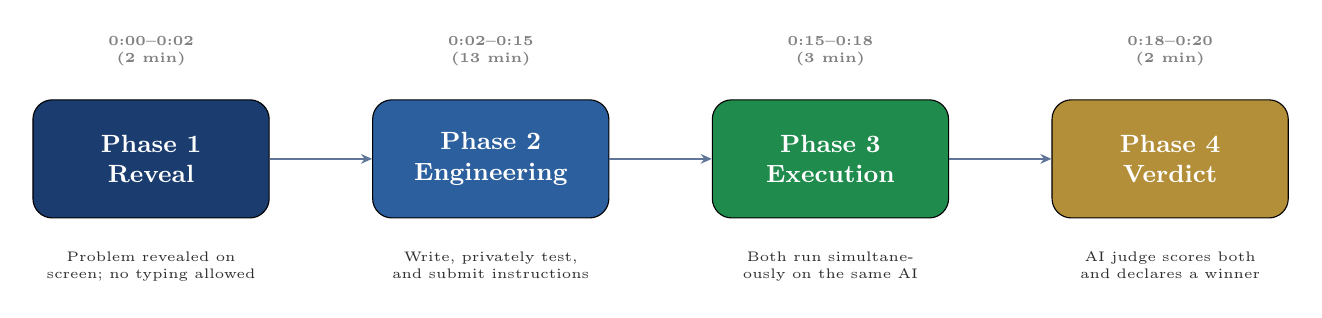
\begin{tikzpicture}[
    phase/.style={draw, rounded corners=7pt, minimum width=3cm, minimum height=1.5cm,
        font=\small\bfseries, align=center, text=white, inner sep=5pt},
    timelab/.style={font=\tiny\bfseries, text=gray, align=center},
    arr/.style={-{Stealth[length=4pt,width=3.5pt]}, line width=1pt, primaryblue!70},
    detail/.style={font=\tiny, text=darktext, align=center, text width=2.9cm},
]
\node[phase, fill=primaryblue]           (p1) {Phase 1\\Reveal};
\node[phase, fill=sectionblue, right=1.3cm of p1]  (p2) {Phase 2\\Engineering};
\node[phase, fill=successgreen!80!black, right=1.3cm of p2] (p3) {Phase 3\\Execution};
\node[phase, fill=accentgold!85!black,   right=1.3cm of p3] (p4) {Phase 4\\Verdict};
\draw[arr] (p1) -- (p2); \draw[arr] (p2) -- (p3); \draw[arr] (p3) -- (p4);
\node[timelab, above=0.3cm of p1] {0:00--0:02\\(2 min)};
\node[timelab, above=0.3cm of p2] {0:02--0:15\\(13 min)};
\node[timelab, above=0.3cm of p3] {0:15--0:18\\(3 min)};
\node[timelab, above=0.3cm of p4] {0:18--0:20\\(2 min)};
\node[detail, below=0.3cm of p1] {Problem revealed on screen; no typing allowed};
\node[detail, below=0.3cm of p2] {Write, privately test, and submit instructions};
\node[detail, below=0.3cm of p3] {Both run simultaneously on the same AI};
\node[detail, below=0.3cm of p4] {AI judge scores both and declares a winner};
\end{tikzpicture}
\caption{The 20-Minute Match Protocol}
\end{figure}

\textbf{Phase 1 --- The Problem Reveal (0:00--0:02):} The Game Master reveals the challenge on the main screen. Both competitors see the exact same problem at the same moment. No typing is permitted during this window.

\textbf{Phase 2 --- The Engineering Phase (0:02--0:15):} Each participant writes the instructions they will give the AI. They may privately test their instructions (up to 5 times) and refine them before submitting. At the 15-minute mark, the platform \textit{automatically locks all submissions}. No extensions are granted.

\begin{tcolorbox}[amberbox, title={The ``Poison Pill'' --- Quarterfinals Onwards}]
From the Quarterfinals (Elite 8) onwards, the Game Master injects a surprise additional constraint at the 7-minute mark. For example: \textit{``Your output must now also be formatted as valid JSON.''} Participants must adapt their instructions to meet both the original and the new requirement in the remaining time. This tests advanced adaptability under pressure.
\end{tcolorbox}

\textbf{Phase 3 --- The Execution (0:15--0:18):} Both sets of instructions are sent to the AI simultaneously, with identical settings for both competitors. Neither gets a head start; neither uses a more capable AI. The AI's responses stream live on the projector, appearing word by word for the audience.

\textbf{Phase 4 --- The Verdict (0:18--0:20):} An independent AI Judge reads the problem statement and both outputs, assigns each a score out of 100, declares the winner, and writes a one-sentence justification. This is entirely automated. The verdict appears on screen within seconds.

\begin{table}[H]
\centering
\renewcommand{\arraystretch}{1.3}
\begin{tabularx}{\textwidth}{>{\bfseries}l c X}
\toprule
Criterion & Weight & What It Means \\
\midrule
Constraint Adherence  & 40\% & Did the AI's output follow every rule stated in the problem? \\
Logic \& Correctness  & 35\% & Is the output factually accurate, logically sound, and well-structured? \\
Elegance \& Efficiency & 25\% & Is the output high quality given the conciseness of the participant's instructions? \\
\bottomrule
\end{tabularx}
\caption{AI Judge Evaluation Criteria (Disclosed to All Participants in Advance)}
\end{table}

If any verdict is contested, the Game Master triggers a second evaluation using a different judge model. All verdicts, including challenged ones, are permanently logged.

% ============================================================================
\section{Tournament Structure: From 50 Players to 1 Champion}
% ============================================================================

\subsection{The Bracket}

The tournament uses standard single-elimination: win and advance, lose and you are out. Because standard brackets work in powers of 2, the 50-player field is structured as follows: \textbf{14 participants} receive a \textit{``bye''} (they skip the opening round and advance directly to the Round of 32), while the remaining \textbf{36 participants} compete in the \textit{Play-In Round} (18 matches). The 18 Play-In winners join the 14 bye-holders in a 32-person bracket, which then plays through Round of 32, Round of 16, Quarterfinals, Semi-Finals, and the Grand Final. Total matches across the entire tournament: \textbf{49}.

\subsection{Wave-Based Execution and Schedule}

With 6 battle stations (2 computers each, 12 total), up to \textbf{6 matches can run simultaneously} per wave.

\begin{table}[H]
\centering
\renewcommand{\arraystretch}{1.3}
\begin{tabularx}{\textwidth}{>{\bfseries}l c c l X}
\toprule
Round & Matches & Waves & Time Slot & Notes \\
\midrule
Play-In Round  & 18 & 3 (6/6/6)   & 10:50--11:25 AM & 8 min each; no Poison Pill. \\
Round of 32    & 16 & 3 (6/6/4)   & 11:30 AM--12:40 PM & 20 min each; full protocol. \\
--- Lunch Break ---  & & & 12:40--1:30 PM & Bracket live on screen. \\
Round of 16    & 8  & 2 (6/2)     & 1:30--2:20 PM & 20 min each; full protocol. \\
Quarterfinals  & 4  & 1 wave of 4 & 2:25--2:50 PM & Poison Pill introduced. \\
Semi-Finals    & 2  & 1 wave of 2 & 2:55--3:20 PM & Live projection for audience. \\
Grand Final    & 1  & 1 match     & 3:25--4:00 PM & Main stage; full audience. \\
Awards         & -- & --          & 4:00--4:30 PM & Prizes and certificates. \\
\midrule
\textbf{Total} & \textbf{49} & \textbf{11 waves} & & \\
\bottomrule
\end{tabularx}
\caption{Round-by-Round Breakdown and Schedule}
\end{table}

% ============================================================================
\section{The AI Components: Plain-Language Explanation}
% ============================================================================

Two completely separate AI models are used: one to \textbf{run} the competition (Battle AI), and one to \textbf{judge} it (Judge AI). They never interact with each other and neither can be influenced by any participant.

\begin{tcolorbox}[greenbox, title={The Battle AI --- ``The Frozen Model'' (What participants compete to control)}]
This is the AI that takes participants' written instructions and produces a response. ``Frozen'' means all settings are locked identically for every participant in every match. The platform uses Groq's \textbf{paid commercial API} to guarantee zero rate-limit interruptions during live matches.

\smallskip
\begin{tabularx}{\linewidth}{@{}>{\bfseries}l X@{}}
Model:    & Llama 3.3 70B (open-source AI from Meta, on Groq's \textit{paid} inference infrastructure) \\
Speed:    & 500--800 words per second --- essential for the 3-minute execution window \\
Pricing:  & INR~50 per million input tokens + INR~67 per million output tokens (pay-per-use) \\
Fairness: & All 50 participants use the identical AI with identical settings, every match. \\
\end{tabularx}
\end{tcolorbox}

\begin{tcolorbox}[purplebox, title={The Judge AI --- The Impartial Evaluator (Separate from everything else)}]
This AI never interacts with participants. Its sole job: read the problem and both outputs, then declare which solved the problem better. Both the primary and fallback judge run on \textbf{paid commercial API tiers} --- no quota throttling during the live event.

\smallskip
\begin{tabularx}{\linewidth}{@{}>{\bfseries}l X@{}}
Primary:      & Gemini 2.0 Flash, Google AI Paid Tier (INR~9/million input + INR~34/million output tokens) \\
Backup:       & GPT-4o-mini via OpenRouter --- activated automatically only if the primary model fails \\
Consistency:  & Receives identical evaluation instructions every match. Criteria never change. \\
Transparency: & The judge's written justification is displayed on screen after every verdict. \\
\end{tabularx}
\end{tcolorbox}

\textbf{Why use an AI Judge instead of human judges?}
\begin{enumerate}[leftmargin=1.2cm, itemsep=2pt]
    \item \textbf{Speed:} With 6 matches running at once, humans cannot evaluate 12 outputs in parallel in 2 minutes. The AI does this in seconds.
    \item \textbf{Consistency:} The AI applies identical criteria every time --- no inter-judge variation.
    \item \textbf{No Bias:} The judge has no knowledge of any participant. It evaluates only the text of the outputs.
    \item \textbf{Audit Trail:} Every verdict is stored as structured data with scores and a written justification --- a permanent record that no verbal judgement can produce.
\end{enumerate}

% ============================================================================
\section{Platform Technology and Infrastructure}
% ============================================================================

\subsection{A Non-Technical Summary of the System}

The platform is a website with three layers. The \textbf{interface} is what opens in a browser: participants open it on their assigned computer and are automatically in their match workspace (no login required); spectators open it and see the public view; the Game Master opens it on a separate machine and sees the admin control panel. The \textbf{processing engine} works invisibly behind the scenes --- routing instructions to the AI, running the judge, updating the bracket, pushing live score updates to all screens, and enforcing timers. The \textbf{data layer} permanently stores everything: participants, prompts, outputs, scores, and Game Master actions, all available for post-event audit or export.

\textbf{How live updates work:} The platform uses a standard technology that pushes updates to every screen simultaneously. When a match result is announced, the bracket on every spectator's screen refreshes automatically within one second, without anyone manually refreshing their browser.

\textbf{How participants are identified:} Each of the 12 competition computers is pre-registered with a unique identity. When a participant checks in, the Game Master assigns them to a computer. That computer automatically has the participant's workspace ready --- no password required. If hardware fails, the Game Master reassigns the participant in under 2 minutes without any data loss.

\subsection{Infrastructure and Cost}
\label{sec:infra}

All cloud services are procured on \textbf{paid, production-grade tiers} to guarantee uptime, SLA coverage, higher rate limits, and commercial support during the event. Costs cover a \textbf{2-month window} (development + live event month) plus one-time API usage. All amounts are in Indian Rupees.

\begin{table}[H]
\centering
\small
\renewcommand{\arraystretch}{1.25}
\begin{tabular}{>{\bfseries}p{3.2cm} p{3.8cm} p{5cm} r}
\toprule
\textbf{Component} & \textbf{Provider \& Plan} & \textbf{Why Paid Tier} & \textbf{INR} \\
\midrule
\multicolumn{4}{l}{\textcolor{sectionblue}{\textbf{Recurring Hosting (billed for 2 months)}}} \\
\midrule
Website Hosting      & Vercel Pro (INR~1,700/mo)       & Production SLA, zero cold-starts, higher bandwidth limits       & 3,400 \\
Live Updates Server  & Railway Hobby (INR~1,700/mo)    & Dedicated resources \& uptime guarantee for WebSocket connections & 3,400 \\
Database             & MongoDB Atlas M2 (INR~1,275/mo) & Automated backups, higher IOPS, 99.9\% availability SLA         & 2,550 \\
Speed Cache          & Upstash Redis (INR~850/mo est.) & No free-tier throttling on high-frequency match timer updates    & 1,700 \\
DDoS \& CDN          & Cloudflare Pro (INR~1,700/mo)   & Web Application Firewall + DDoS mitigation for public platform   & 3,400 \\
\midrule
\multicolumn{4}{l}{\textcolor{warnamber!80!black}{\textbf{One-Time Event API Usage (with safety buffer)}}} \\
\midrule
Battle AI            & Groq Paid API                   & Llama~3.3 70B; 5$\times$ buffer on 350+ calls for dev \& live rounds & 2,125 \\
Judge AI (Primary)   & Google AI Paid Tier             & Gemini~2.0 Flash; 10$\times$ buffer on 100+ evaluations          & 1,275 \\
Fallback Judge       & OpenRouter GPT-4o-mini          & Emergency backup; activated only if primary judge fails          &   850 \\
Domain Registration  & Cloudflare Registrar (1 yr)     & Custom domain --- e.g.\ promptwars.technous.in                  & 1,275 \\
\midrule
\multicolumn{3}{r}{\textbf{Total Platform Infrastructure Budget}} & \textbf{27,125} \\
\multicolumn{3}{r}{\textit{(rounded for budget submission)}} & \textit{\textbf{$\approx$ INR~28,000}} \\
\bottomrule
\end{tabular}
\caption{Infrastructure Budget --- Paid Production Tiers (2-Month Window, All Amounts in INR)}
\end{table}

\begin{tcolorbox}[highlightbox]
\centering
{\normalsize\bfseries\textcolor{primaryblue}{Total Platform Infrastructure Budget: INR~28,000}}\\[0.12cm]
{\small Covers 2 months of paid production hosting + all AI API usage with generous safety buffers.}\\[0.08cm]
{\small All services carry commercial SLAs --- no dependency on free-tier quotas during the live event.}
\end{tcolorbox}

% ============================================================================
\section{Transparency, Security, and Contingency}
% ============================================================================

\subsection{Transparency Guarantees}

\begin{itemize}[leftmargin=1.2cm, itemsep=2pt]
    \item All judge verdicts are permanently stored: full output text, scores for each player, and written justification.
    \item All Game Master actions are timestamped and logged. Any override or intervention is on record.
    \item The judge's evaluation criteria (40/35/25 weightings) are published to all participants before the event. There are no secret scoring rules.
    \item A full data export is available after the event for review by any authorised party.
    \item The live leaderboard is visible to everyone throughout the event; any participant can see their own results at any time.
\end{itemize}

\subsection{Physical Requirements at the Venue}

\begin{table}[H]
\centering
\renewcommand{\arraystretch}{1.3}
\begin{tabularx}{\textwidth}{>{\bfseries}l X}
\toprule
Requirement & Details \\
\midrule
12 Competition Computers & 2 per station, 6 stations. The existing lab PCs in AI Block Lab~201. No participant hardware needed. \\
1 Game Master Computer   & Dedicated machine for the coordinator's admin console. \\
3--5 Backup Laptops      & On standby. If any station PC fails, participant is transferred without data loss in under 2 minutes. \\
Internet Connection      & Dedicated high-speed Wi-Fi (min.\ 100 Mbps). 4G/5G mobile hotspot kept on standby as backup. \\
Projector / LED Screen   & For Semi-Finals and Grand Final live projection. Minimum 3000 lumens, HDMI connection. \\
Power Strips             & 4--6 multi-socket strips for all station computers and peripherals. \\
\bottomrule
\end{tabularx}
\caption{Physical Infrastructure Requirements}
\end{table}

\subsection{Contingency Planning}

\begin{table}[H]
\centering
\renewcommand{\arraystretch}{1.3}
\begin{tabularx}{\textwidth}{>{\bfseries}l c X}
\toprule
Risk & Probability & Mitigation \\
\midrule
Internet outage            & Medium & Mobile hotspot activated immediately; critical services pre-cached locally. \\
Station computer fails     & Low    & Participant moved to standby laptop in $<$2 minutes; session transferred, no data lost. \\
AI API becomes unavailable & Low    & Platform auto-switches to backup provider. No manual action needed from any team member. \\
Participant does not show  & Medium & Waitlist fills spots; bracket adjusted with automatic byes. \\
AI Judge gives unclear verdict & Low & Game Master triggers second evaluation from a different model. All verdicts logged regardless. \\
Schedule runs over time    & Medium & Automated timers enforce match cutoffs. Play-In round can be shortened to recover time. \\
\bottomrule
\end{tabularx}
\caption{Risk and Mitigation Matrix}
\end{table}

% ============================================================================
\section{Operational Team and Financials}
\label{sec:team}
% ============================================================================

\begin{table}[H]
\centering
\renewcommand{\arraystretch}{1.3}
\begin{tabularx}{\textwidth}{>{\bfseries}l c X}
\toprule
Role & Count & Responsibilities \\
\midrule
Event Coordinator    & 1   & Overall schedule management, escalation handling. \\
Game Master          & 1--2 & Operates admin console, reveals problems, manages timers, announces results. \\
Technical Lead       & 1   & Manages cloud credentials, monitors platform health, troubleshoots issues. \\
Station Supervisors  & 2--3 & Oversee battle stations, ensure submission across all active matches. \\
Leaderboard Manager  & 1   & Monitors live bracket; maintains backup leaderboard. \\
Floor Volunteers     & 3--4 & Assist participants, manage seating, handle questions. \\
Registration Desk    & 1--2 & Check-in, identity verification, station assignment coordination. \\
\midrule
\textbf{Total} & \textbf{10--14} & \\
\bottomrule
\end{tabularx}
\caption{Event Team Structure}
\end{table}

\begin{table}[H]
\centering
\renewcommand{\arraystretch}{1.3}
\begin{tabularx}{\textwidth}{>{\bfseries}l X r}
\toprule
Item & Details & Amount (INR) \\
\midrule
\multicolumn{2}{l}{\textcolor{successgreen}{\textbf{Revenue}}} \\
Registration Fees  & 50 participants $\times$ INR~169 & 8,450 \\
\midrule
\multicolumn{2}{l}{\textcolor{alertred}{\textbf{Expenditure}}} \\
1st Place Prize    & Winner                                    & 7,000 \\
2nd Place Prize    & Runner-up                                 & 5,000 \\
3rd Place Prize    & Semi-finalist                             & 3,000 \\
Platform Infrastructure & Vercel Pro + Railway Pro + MongoDB Atlas + Redis + Cloudflare + AI APIs + Domain (see Section~\ref{sec:infra} for full breakdown) & 28,000 \\
Certificates \& Printing & Participant and winner materials    & 500 \\
\midrule
\textbf{Total Expenditure} & & \textbf{43,500} \\
\textbf{Net from Fest Budget} & Prize pool + platform + shortfall (after registration offset) & \textbf{35,050} \\
\bottomrule
\end{tabularx}
\caption{Financial Overview}
\end{table}

% ============================================================================
\section{Summary and Approval Request}
% ============================================================================

The PromptWars Platform is a fully designed, well-tested, and cost-effective system that eliminates manual error, guarantees consistent and transparent automated judging, and manages the entire competitive lifecycle --- from participant registration to grand champion announcement --- with a \textbf{total platform infrastructure budget of INR~28,000} covering two months of paid production services and all AI API usage. The event operates within existing university lab resources and requires no specialised hardware purchases.

\begin{tcolorbox}[greenbox, title={Formal Approval Requested For}]
\begin{enumerate}[leftmargin=1cm, itemsep=3pt]
    \item \textbf{Venue:} AI Block --- Lab~201 for the full event day (Day~2 of GLITCH Tech Fest 2026, March 15, 2026).
    \item \textbf{Infrastructure:} Use of 12 lab PCs, projector, and dedicated internet access.
    \item \textbf{Prize Budget:} INR~15,000 prize pool allocation from the GLITCH Tech Fest 2026 fund.
    \item \textbf{Platform Budget:} INR~28,000 for paid production-grade cloud hosting and AI API usage (full breakdown in Section~\ref{sec:infra}).
    \item \textbf{Personnel:} Authorisation for 10--14 volunteers to operate the event.
\end{enumerate}
\end{tcolorbox}

\vspace{1cm}

\begin{tabularx}{\textwidth}{X X}
\textbf{Prepared By:} & \textbf{Approved By:} \\[1.2cm]
\rule{5.5cm}{0.5pt} & \rule{5.5cm}{0.5pt} \\
The Technous Club --- Event Committee & {[Name / Designation]} \\
Date: \rule{2.8cm}{0.5pt} & Date: \rule{2.8cm}{0.5pt} \\[1.1cm]
\textbf{Reviewed By (Faculty Advisor):} & \textbf{Endorsed By (HOD / Dean):} \\[1.2cm]
\rule{5.5cm}{0.5pt} & \rule{5.5cm}{0.5pt} \\
{[Faculty Advisor Name]} & {[HOD / Dean Name]} \\
Date: \rule{2.8cm}{0.5pt} & Date: \rule{2.8cm}{0.5pt} \\
\end{tabularx}

\vfill
\begin{center}
\textcolor{accentgold}{\rule{0.55\textwidth}{1.5pt}}\\[0.45cm]
{\large\bfseries\textcolor{primaryblue}{``Build the Arena. Let the Prompts Decide.''}}\\[0.4cm]
\textcolor{gray}{\rule{0.3\textwidth}{0.5pt}}\\[0.3cm]
\textcolor{gray}{\small\textit{This document is confidential and intended for internal administrative review only.}}\\
\textcolor{gray}{\small\textit{GLITCH Tech Fest 2026 --- The Technous Club, Shoolini University of Biotechnology and Management Sciences.}}
\end{center}


\newpage
% ============================================================================
\section*{Appendix A: Verified Pricing Evidence}
\addcontentsline{toc}{section}{Appendix A: Verified Pricing Evidence}
% ============================================================================

All infrastructure costs in this document are based on publicly listed official pricing from each provider's pricing page. This appendix documents the verified source, official quoted price, and conversion for each line item. Conversion rate used throughout: \textbf{\$1 USD = INR~85}.

\subsection*{A1. Website Hosting --- Vercel Pro}

\begin{tcolorbox}[greenbox, title={Vercel Pro Plan --- Official Pricing}]
\begin{tabularx}{\linewidth}{@{}>{\bfseries}l X@{}}
Official Price:  & \$20 per seat per month \\
Budgeted (2 mo): & \$40 = INR~3,400 \\
Source URL:      & \texttt{https://vercel.com/pricing} \\
Official Quote:  & \textit{``Pay only for Developer seats (\$20/mo). Each month starts with \$20 in flexible credit.''} \\
                 & --- Vercel Docs, \texttt{vercel.com/docs/plans/pro-plan} \\
\end{tabularx}
\end{tcolorbox}

\subsection*{A2. Live Updates Server --- Railway Pro}

\begin{tcolorbox}[greenbox, title={Railway Pro Plan --- Official Pricing}]
\begin{tabularx}{\linewidth}{@{}>{\bfseries}l X@{}}
Official Price:  & \$20 per month (Pro plan; includes \$20 in resource usage credit) \\
Budgeted (2 mo): & \$40 = INR~3,400 \\
Source URL:      & \texttt{https://railway.com/pricing} \\
Official Quote:  & \textit{``Pro is for professional developers and their teams shipping to production. The Pro plan includes \$20 of resource usage per month.''} \\
                 & --- Railway Pricing Docs, \texttt{docs.railway.com/reference/pricing/plans} \\
\end{tabularx}
\end{tcolorbox}

\subsection*{A3. Database --- MongoDB Atlas M10}

\begin{tcolorbox}[greenbox, title={MongoDB Atlas M10 Dedicated Cluster --- Official Pricing}]
\begin{tabularx}{\linewidth}{@{}>{\bfseries}l X@{}}
Official Price:  & \$57/month (M10 dedicated cluster, AWS US-East, 10~GB storage, 2~vCPUs) \\
Budgeted (2 mo): & INR~4,850/mo $\times$ 2 = INR~9,700 \\
Source URL:      & \texttt{https://www.mongodb.com/pricing} \\
Official Quote:  & \textit{``Dedicated Tier: Starting at \$57 monthly for M10 clusters.''} \\
                 & --- MongoDB Atlas Pricing, \texttt{mongodb.com/pricing} \\
\end{tabularx}
\end{tcolorbox}

\subsection*{A4. Speed Cache --- Upstash Redis (Pay-as-you-go)}

\begin{tcolorbox}[greenbox, title={Upstash Redis --- Official Pricing}]
\begin{tabularx}{\linewidth}{@{}>{\bfseries}l X@{}}
Official Price:  & Pay-as-you-go: \$0.20 per 100,000 requests; free tier includes 500K commands/month \\
Budgeted:        & \$10/mo est.\ $\times$ 2 months = INR~1,700 (generous buffer for high-frequency timer ticks) \\
Source URL:      & \texttt{https://upstash.com/pricing/redis} \\
Official Quote:  & \textit{``Free Tier now includes 500K commands per month. Beyond that, \$0.20 per 100,000 requests.''} \\
                 & --- Upstash Blog, \texttt{upstash.com/blog/redis-new-pricing} (March 2025) \\
\end{tabularx}
\end{tcolorbox}

\subsection*{A5. DDoS Protection \& CDN --- Cloudflare Pro}

\begin{tcolorbox}[greenbox, title={Cloudflare Pro Plan --- Official Pricing}]
\begin{tabularx}{\linewidth}{@{}>{\bfseries}l X@{}}
Official Price:  & \$25/month (monthly billing) or \$20/month effective (\$240/year, annual billing) \\
Budgeted (2 mo): & \$40 = INR~3,400 (at annual-equivalent rate of \$20/mo) \\
Source URL:      & \texttt{https://www.cloudflare.com/plans/pro/} \\
Official Quote:  & \textit{``Pro plan: \$240 per year for annual billing (the equivalent of \$20 per month).''} \\
                 & --- Cloudflare Community FAQ, \texttt{community.cloudflare.com} \\
\end{tabularx}
\end{tcolorbox}

\subsection*{A6. Battle AI --- Groq Cloud (Llama 3.3 70B, Paid API)}

\begin{tcolorbox}[purplebox, title={Groq Paid API --- Llama 3.3 70B Versatile --- Official Pricing}]
\begin{tabularx}{\linewidth}{@{}>{\bfseries}l X@{}}
Official Price:  & \$0.59 per million input tokens + \$0.79 per million output tokens \\
                 & (INR~50 / million input tokens + INR~67 / million output tokens) \\
Budgeted:        & \$25 = INR~2,125 (covers 350+ API calls with 5$\times$ safety buffer for dev + live rounds) \\
Source URL:      & \texttt{https://groq.com/pricing} \\
Official Quote:  & \textit{``Llama 3.3 70B Versatile 128k --- Input: \$0.59 per million tokens. Output: \$0.79 per million tokens.''} \\
                 & --- Groq Official Pricing Page \\
\end{tabularx}
\end{tcolorbox}

\subsection*{A7. Judge AI (Primary) --- Google Gemini 2.0 Flash (Paid Tier)}

\begin{tcolorbox}[purplebox, title={Google Gemini 2.0 Flash API --- Official Pricing (Paid Tier)}]
\begin{tabularx}{\linewidth}{@{}>{\bfseries}l X@{}}
Official Price:  & \$0.10 per million input tokens + \$0.40 per million output tokens (text/image/video) \\
                 & (INR~9 / million input tokens + INR~34 / million output tokens) \\
Budgeted:        & \$15 = INR~1,275 (covers 100+ judge evaluations with 10$\times$ safety buffer) \\
Source URL:      & \texttt{https://ai.google.dev/gemini-api/docs/pricing} \\
Official Quote:  & \textit{``Gemini 2.0 Flash --- Paid Tier: Input: \$0.10 (text/image/video). Output: \$0.40 per 1M tokens.''} \\
                 & --- Google AI for Developers Pricing Docs \\
\end{tabularx}
\end{tcolorbox}

\subsection*{A8. Fallback Judge --- OpenRouter GPT-4o-mini}

\begin{tcolorbox}[purplebox, title={OpenRouter GPT-4o-mini --- Reference Pricing}]
\begin{tabularx}{\linewidth}{@{}>{\bfseries}l X@{}}
Official Price:  & \$0.15 per million input tokens + \$0.60 per million output tokens (via OpenRouter) \\
Budgeted:        & \$10 = INR~850 (emergency reserve; only triggered if primary judge model fails) \\
Source URL:      & \texttt{https://openrouter.ai/openai/gpt-4o-mini} \\
Note:            & Budget is a precautionary reserve. Actual spend depends on number of fallback activations. \\
\end{tabularx}
\end{tcolorbox}

\subsection*{A9. Domain Registration --- Cloudflare Registrar}

\begin{tcolorbox}[greenbox, title={Cloudflare Registrar --- Domain Registration}]
\begin{tabularx}{\linewidth}{@{}>{\bfseries}l X@{}}
Official Price:  & At-cost pricing; .in domains approximately INR~900--1,200 per year \\
Budgeted:        & \$15 = INR~1,275 (1-year registration with buffer for .com fallback if .in unavailable) \\
Source URL:      & \texttt{https://www.cloudflare.com/products/registrar/} \\
Note:            & Cloudflare Registrar offers no-markup, at-cost pricing with no hidden renewal fees. \\
\end{tabularx}
\end{tcolorbox}

\vspace{0.4cm}
\begin{tcolorbox}[highlightbox]
\centering
{\small\bfseries All prices above are from official vendor pricing pages as of the time of document preparation.}\\[0.1cm]
{\small Budget figures include generous safety buffers for testing, retries, and unexpected usage spikes.}\\[0.1cm]
{\small Where a range exists (e.g.\ monthly vs.\ annual billing), the more cost-effective option is used in the budget.}
\end{tcolorbox}

\end{document}
